%%% Notes on nitrogen CCSN and AGB star yields of N %%% 

\providecommand{\main}{..} 
\documentclass[\main/notes.tex]{subfiles} 

\begin{document} 
\begin{center} 
\textbf{{\Large CCSN and AGB Star Yields of Nitrogen}} 
\end{center} 

\noindent 
{\Large \textit{Core-Collapse Supernova Yields}} 
\par\noindent 
Empirically, nitrogen-to-oxygen ratios exhibit a plateau at 
$\log$(N/O)~$\approx$~-1.5 for~$\log$(O/H)~$\lesssim$~8 (see Fig. 1 of 
\citealp{Vincenzo2016} comparing~\citealp{Berg2012},~\citealp*{Izotov2012}, and 
\citealp{James2015} measurements). 
\twolineskip 
\textbf{What is the implied relation between the IMF integrated CCSN yields of 
nitrogen and oxygen?} 
\par\noindent 
The ratio of their yields can be related to the number densities of the two 
nuclei in the supernova ejecta via: 
\begin{equation} 
\ddfrac{y_\text{N}^\text{CC}}{y_\text{O}^\text{CC}} = 
\ddfrac{\mu_\text{N}n_\text{N}}{\mu_\text{O}n_\text{O}} 
\end{equation} 
where~$\mu_x$~is the mean molecular weight of a species~$x$~and~$n_x$ is the 
number of nuclei. Taking the ratio~$n_\text{N}/n_\text{O}$~from these observed 
results yields: 
\begin{equation} 
\ddfrac{y_\text{N}^\text{CC}}{y_\text{O}^\text{CC}} = 
\ddfrac{\mu_\text{N}}{\mu_\text{O}}10^{\log\text{(N/O)}} 
\end{equation} 
Though supernova ejecta may produce different isotopic ratios of N than AGB 
stars, potentially  
altering the ratio~$\mu_\text{N}/\mu_\text{O}$, taking~$\mu_\text{N}$ = 14.007 
and~$\mu_\text{O}$ = 15.999 from a periodic table suggests that, with the 
previously adopted~$y_\text{O}^\text{CC}$ = 0.015 (e.g.~\citealp*{Weinberg2017}; 
\citealp{Johnson2020}), this suggests 
\begin{equation} 
y_\text{N}^\text{CC} = \ddfrac{\mu_\text{N}}{\mu_\text{O}}10^{\log\text{(N/O)}} 
y_\text{O}^\text{CC} = \ddfrac{14.007}{15.999}10^{-1.5}(0.015) \approx 
4.15\times10^{-4} 
\end{equation} 
\twolineskip 
\textbf{Can this be understood from theoretically predicted yields?} 

\begin{figure}[!t] 
\centering 
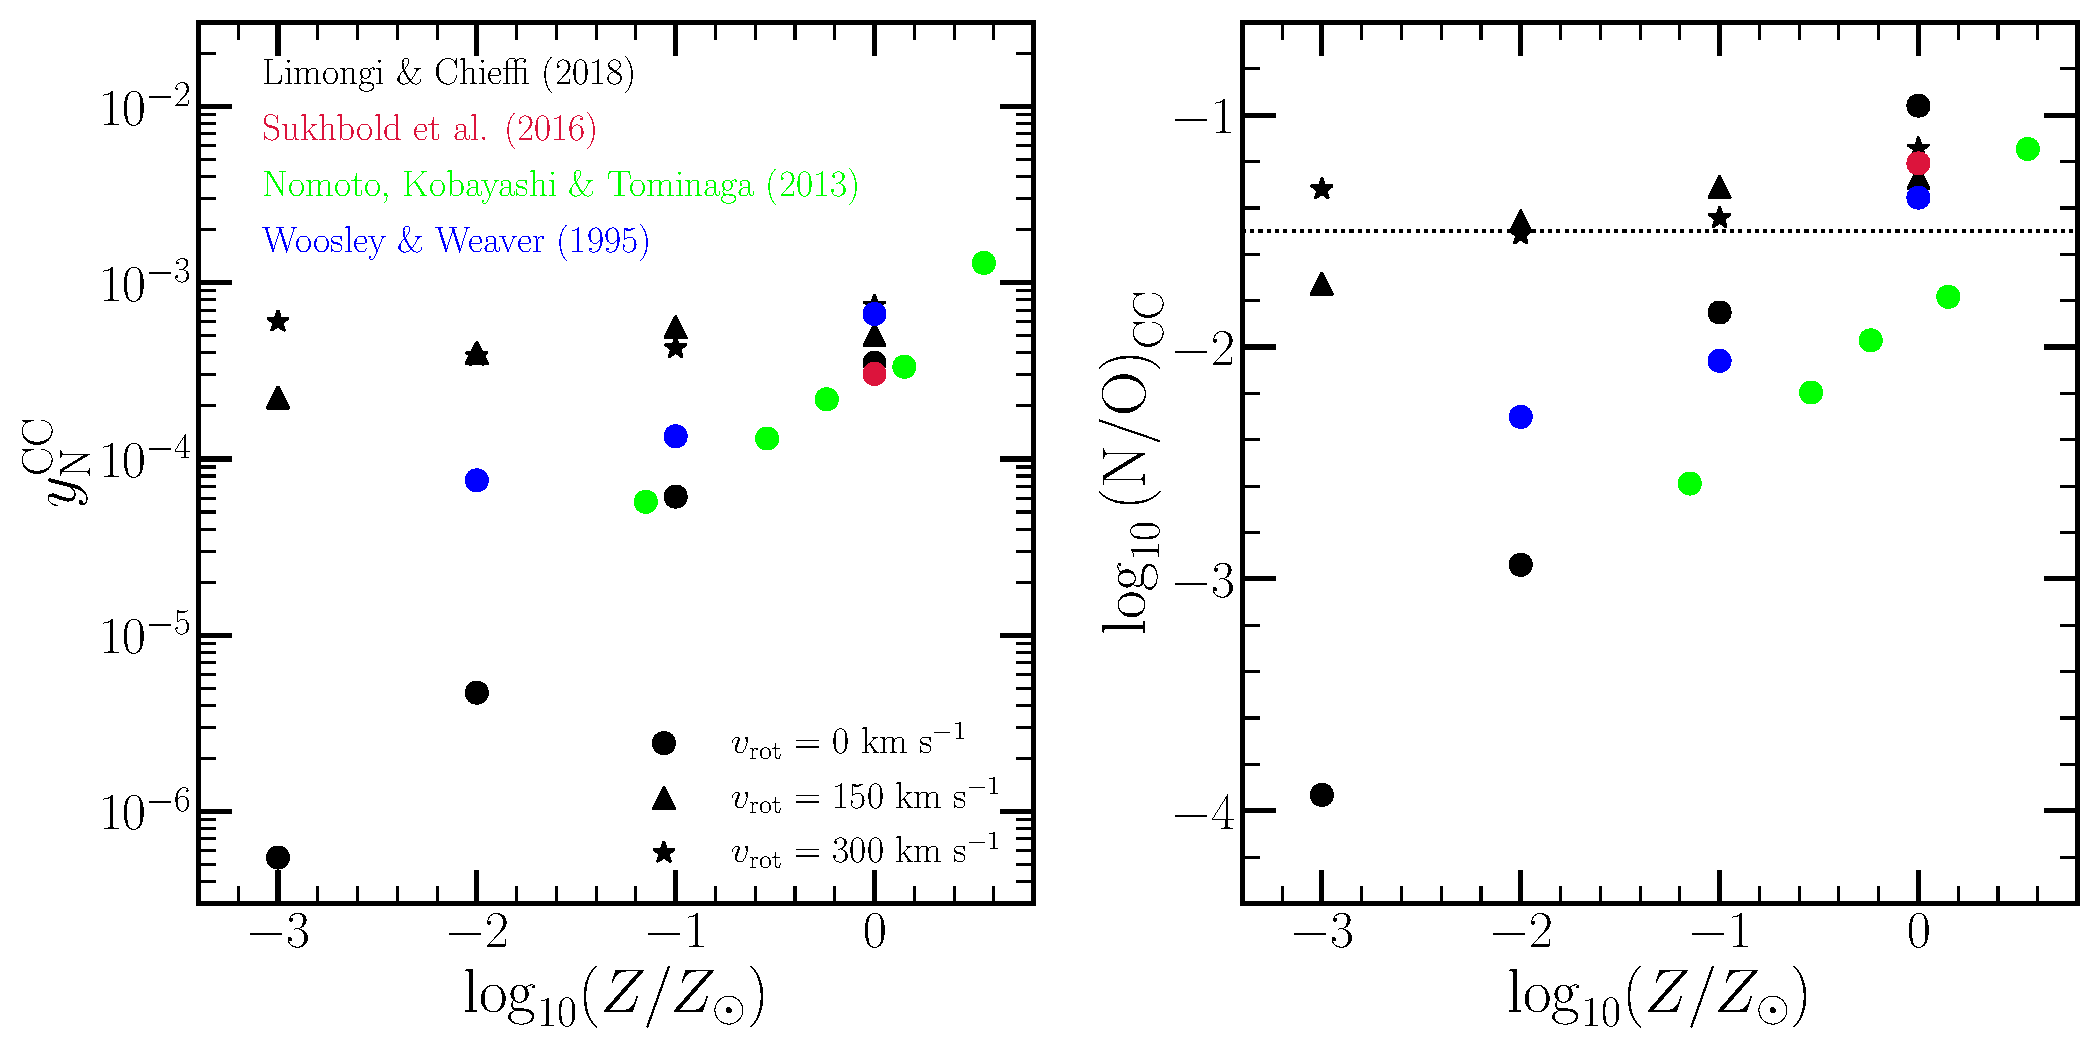
\includegraphics[scale = 0.7]{\main/yields/n_cc_yields.pdf} 
\caption{IMF-integrated CCSN yields of N computed with VICE using the 
\citet{Limongi2018} (black),~\citet{Sukhbold2016} (crimson),~\citet{Nomoto2013} 
(lime), and~\citet{Woosley1995} (blue) yield sets. The~\citet{Limongi2018} 
yields are calculated with progenitor rotational velocities of 
$v_\text{rot}$ = 0 (circles), 150 (triangles), and 300 km/s (stars). All other 
studies only report yields for non-rotating progenitors. } 
\label{fig:n_cc_yields} 
\end{figure} 

\noindent 
Figure~\ref{fig:n_cc_yields} presents the IMF-integrated yields 
$y_\text{N}^\text{CC}$~computing with VICE using the~\citet{Limongi2018}, 
\citet{Sukhbold2016},~\citet{Nomoto2013}, and~\citet{Woosley1995} CCSN yield 
tables, with~\citet{Limongi2018} being the only study which reports yields for 
rotating progenitors. Broadly, the non-rotating predictions are consistent with 
one another, and predict a significant metallicity dependence; the lowest 
metallicity progenitor from~\citet{Woosley1995} predicts a somewhat higher 
yield at~$\log_{10}(Z/Z_\odot)$ = -2, but this is the only outlier. The 
rotating progenitors from~\citet{Limongi2018}, however, predict that the 
yield should be considerably enhanced by rotation. They interpret this as being 
due to the interplay between the core helium and hydrogen burning shells 
triggered by rotation-induced instabilities, which drives the synthesis of all 
products of CNO, not just~$^{14}$N (see their abstract). These yields predict a 
relatively metallicity-independent~$y_\text{N}^\text{CC}$ of 
$\sim5\times10^{-4}$, in surprisingly good agreement with the empirically 
derived value of~$4.15\times10^{-4}$. 

\newpage\noindent 
\textbf{What is the implied plateau in [N/O]?} 
\par\noindent 
[N/O] and~$\log$(N/O) are directly related, but one is relative to the sun 
while the other is just a ratio of number densities. Expanding [N/O]: 
\begin{subequations}\begin{align} 
\text{[N/O]} &= \text{[N/H]} - \text{[O/H]} \\ 
&= \log_{10}\left(\ddfrac{Z_\text{N}}{Z_{\text{N},\odot}}\right) - 
\log_{10}\left(\ddfrac{Z_\text{O}}{Z_{\text{O},\odot}}\right) 
\\ 
&= \log_{10}\left(\ddfrac{Z_\text{N}}{Z_\text{O}}\right) - \log_{10}\left(
\ddfrac{Z_{\text{N},\odot}}{Z_{\text{O},\odot}}\right) 
\end{align}\end{subequations} 
Zooming in on the~$Z_\text{N}/Z_\text{O}$ term: 
\begin{subequations}\begin{align} 
\log_{10}\left(\ddfrac{Z_\text{N}}{Z_\text{O}}\right) &= 
\log_{10}\left(\ddfrac{\mu_\text{N}n_\text{N}}{\mu_\text{O}n_\text{O}}\right) \\ 
&= \log_{10}\left(\ddfrac{\mu_\text{N}}{\mu_\text{O}}\right) + \log_{10}\left(
\ddfrac{n_\text{N}}{n_\text{O}}\right) 
\end{align}\end{subequations} 
where~$\mu$~and~$n$~are again the mean molecular weight and number of some 
species~$x$. The term~$\log_{10}\left(n_\text{N}/n_\text{O}\right)$~is exactly 
the~$\log$(N/O) value which~\citet{Berg2012},~\citet*{Izotov2012}, and 
\citet{James2015} measured to be~$\sim$-1.5. Plugging this in: 
\begin{subequations}\begin{align} 
\text{[N/O]} &= \log_{10}\left(\ddfrac{\mu_\text{N}}{\mu_\text{O}}\right) + 
\log_{10}\left(\ddfrac{n_\text{N}}{n_\text{O}}\right) - \log_{10}\left(
\ddfrac{Z_{\text{N},\odot}}{Z_{\text{O},\odot}}\right) 
\end{align}\end{subequations} 
Taking~$\mu_\text{N}$~= 14.007 and~$\mu_\text{O}$~= 15.999 again, with the 
empirical result of~$\log_{10}\left(n_\text{N}/n_\text{O}\right)$~= -1.5 and 
the~\citet{Asplund2009} solar photospheric composition of~$Z_{\text{N},\odot}$ 
= $6.91\times10^{-4}$~and~$Z_{\text{O},\odot}$~= 0.00572, yields the following: 
\begin{equation} 
\text{[N/O]}_\text{plateau} = -0.64 
\end{equation} 

\twolineskip 
{\Large \textit{Asymptotic Giant Branch Star Yields}} 
\par\noindent 
Figure~\ref{fig:n_agb_yields} presents the fractional yields of N as a function 
of progenitor zero age main sequence (ZAMS) mass and metallicity as reported in 
the FRUITY database~\citep{Cristallo2011} and by~\citet{Karakas2010}. Both 
models show the metallicity-dependent nature of seconday nitrogen production, 
whose fractional yields increase with progenitor mass at fixed metallicity. 
Secondary nitrogen production refers to the production of~$^{14}$N at the 
expense of C and O in the CNO cycle; the nuclear reaction network of the CNO 
cycle: 

\twolineskip 
$^{12}$C(p,$\gamma$)$^{13}$N(,$\beta^+$)$^{13}$C(p,$\gamma$)$^{14}$N(p,$\gamma$)
$^{15}$O(,$\beta^+$)$^{15}$N(p,$\alpha$)$^{12}$C 

\twolineskip 
In this chain, the~$^{14}$N(p,$\gamma$)$^{15}$O reaction is particularly slow, 
and for this reason, the net effect of the CNO cycle is to turn all of the C 
and O into~$^{14}$N at their expense. 
\par 
By omparing the left- and right-hand panels of Fig.~\ref{fig:n_agb_yields}, 
it's clear that the~\citet{Karakas2010} predicts secondary nitrogen production 
to be a much stronger effect than~\citet{Cristallo2011}; the yields from high 
mass stars are over an order magnitude larger in~\citet{Karakas2010} than in 
\citet{Cristallo2011} at all reported metallicities except solar. 
\citet{Karakas2010} also predicts a much more complicated mass-dependence than 
does~\citet{Cristallo2011}. {\color{red} Intuitively, I would think that 
secondary N yields should be nothing but monotonic with metallicity. Rotation 
may induce some interesting effects, but unfortunately the~\citet{Karakas2010} 
paper makes no mention of rotation. They were primarily interested in the 
effect of updates to the~$^{13}$C($\alpha$,n)$^{16}$O reaction on light-element 
nucleosynthesis. I'm assuming this means they were using non-rotating models, 
but if this ends up being discussed in a paper I should email Amanda Karakas 
to verify. } 

\begin{figure}[!t]
\centering 
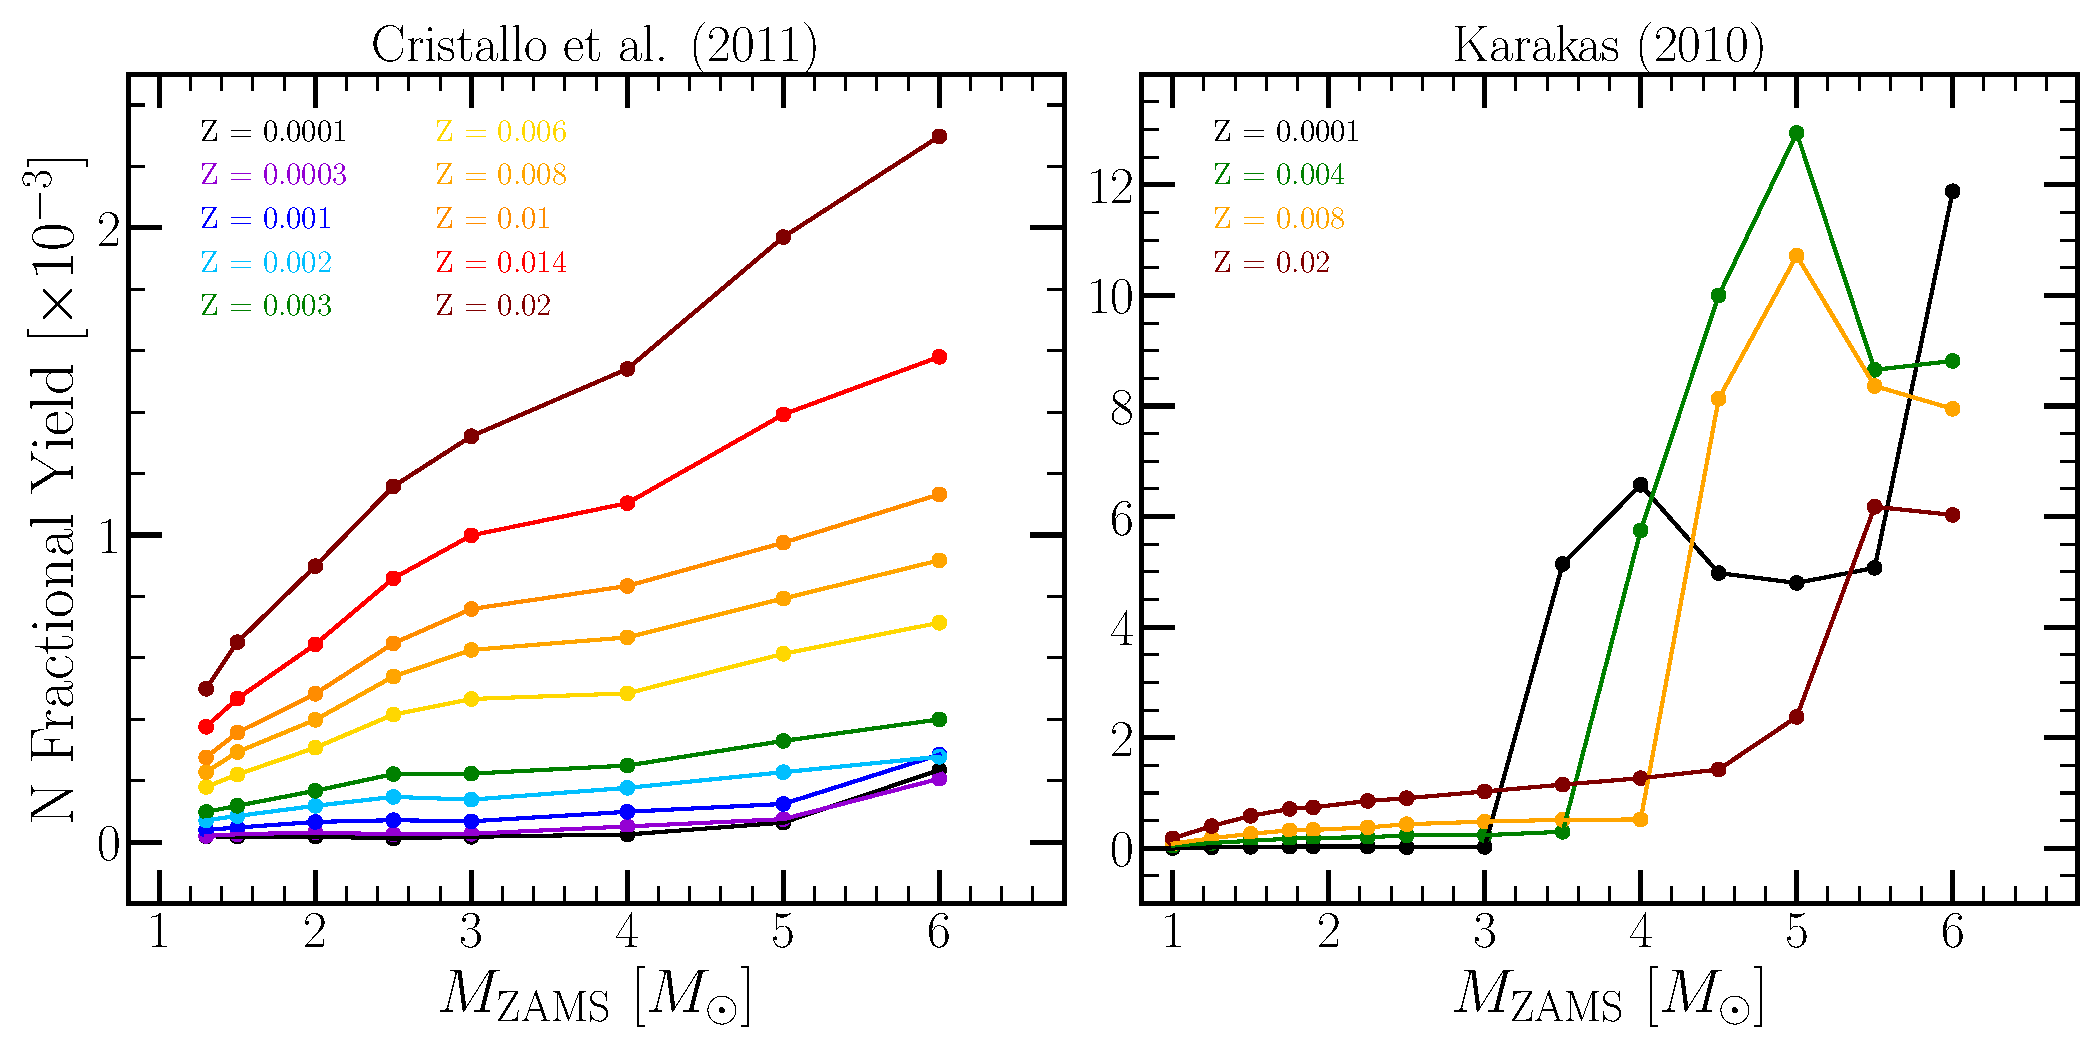
\includegraphics[scale = 0.45]{\main/yields/n_agb_yields.pdf} 
\caption{Fractional yields of N as a function of progenitor zero age main 
sequence mass at the metallicities at which~\citet{Cristallo2011} (left) and 
\citet{Karakas2010} report yields.} 
\label{fig:n_agb_yields} 
\end{figure} 

% \bibliographystyle{mnras}  
% \bibliography{\main/notes} 
\biblio 

\end{document} 

